% Template for Cogsci submission with R Markdown

% Stuff changed from original Markdown PLOS Template
\documentclass[10pt, letterpaper]{article}

\usepackage{cogsci}
\usepackage{pslatex}
\usepackage{float}
\usepackage{caption}

% amsmath package, useful for mathematical formulas
\usepackage{amsmath}

% amssymb package, useful for mathematical symbols
\usepackage{amssymb}

% hyperref package, useful for hyperlinks
\usepackage{hyperref}

% graphicx package, useful for including eps and pdf graphics
% include graphics with the command \includegraphics
\usepackage{graphicx}

% Sweave(-like)
\usepackage{fancyvrb}
\DefineVerbatimEnvironment{Sinput}{Verbatim}{fontshape=sl}
\DefineVerbatimEnvironment{Soutput}{Verbatim}{}
\DefineVerbatimEnvironment{Scode}{Verbatim}{fontshape=sl}
\newenvironment{Schunk}{}{}
\DefineVerbatimEnvironment{Code}{Verbatim}{}
\DefineVerbatimEnvironment{CodeInput}{Verbatim}{fontshape=sl}
\DefineVerbatimEnvironment{CodeOutput}{Verbatim}{}
\newenvironment{CodeChunk}{}{}

% cite package, to clean up citations in the main text. Do not remove.
\usepackage{cite}

\usepackage{color}

% Use doublespacing - comment out for single spacing
%\usepackage{setspace}
%\doublespacing


% % Text layout
% \topmargin 0.0cm
% \oddsidemargin 0.5cm
% \evensidemargin 0.5cm
% \textwidth 16cm
% \textheight 21cm

\title{Order effects in active and passive hypothesis testing}


\author{{\large \bf Kyle MacDonald} \\ \texttt{kyle.macdonald@university.edu} \\ Department of Psychology \\ Stanford University \And {\large \bf Michael C. Frank} \\ \texttt{mcfrank@university.edu} \\ Department of Psychology \\ Stanford University}

\begin{document}

\maketitle

\begin{abstract}
Active learning can speed concept learning by allowing people to collect
highly informative samples based on their current hypotheses. But
real-world learning often involves both active and passive learning
contexts, an interaction that we know little about. In three category
learning experiments with adults, we explore the effectiveness of active
learning in a well-understood category learning task. Experiments 1a and
1b are direct replications of the active learning advantage found in
Markant \& Gureckis (2014). Experiment 2 is an extension that tests how
different sequences of active/passive training modulate the
effectiveness of active learning. Experiment 3 is a conceptual
replication of the order effect findings, using a novel paradigm where
participants learn a higher dimensional concept. Across all experiments,
active training lead to better learning of the target category boundary.
Passive-then-active training was more effective compared to Active-
then-passive in both Experiments 2 and 3. Our replication data provides
additional support that active learning can provide an advantage over
passive learning, and our extension data show that active learning can
be more effective when the learner already has some passive experience
with the learning task.

\textbf{Keywords:}
active learning, hypothesis testing, category learning, replication,
order effects
\end{abstract}

\section{Introduction}\label{introduction}

\begin{itemize}
\item
  What is active learning?
\item
  Why is active learning helpful?

  \begin{itemize}
  \itemsep1pt\parskip0pt\parsep0pt
  \item
    Human active
  \item
    Machine active learning
  \item
    When is active learning most effective
  \end{itemize}
\item
  Current work
\end{itemize}

In their experiment, Markant \& Gureckis (2014) compared the
effectiveness of active vs.~passive training on the rate of
participants' category learning. They tested two different types of
category structures: a Rule-Based (RB) category, which varied along one
dimension, and an Information-Integration (II) category, which varied
along two dimensions. In the active learning condition, learners were
allowed to choose specific observations from the category to test their
beliefs; whereas in passive learning condition, the learner had no
control over what data they saw. They found that participants in the
active condition learned the category structure faster and achieved a
higher overall accuracy rate compared to participants in the passive
learning condition, but this advantage only held for the less complex,
RB category structure.

\section{Experiment 1a}\label{experiment-1a}

Experiment 1a is a direct replication of the advantage for active
learning over passive learning found in Markant \& Gureckis (2014). We
tested participants' category learning for the RB category structure
after receiving either Active or Passive training. We used the same
stimuli and followed the exact procedures as the original study
(described below). All of the stimuli and the experiments can be viewed
and downloaded at the project page for this paper:
\url{https://kemacdonald.github.io/Act-Learn/}.

\subsection{Methods}\label{methods}

\subsubsection{Power analysis}\label{power-analysis}

We calculated Cohen's d for the t-test comparing participants' overall
accuracy rate in the Active and Passive training conditions (d = 0.47).
Next, we performed a post hoc power analysis and found that the original
study achieved a power of 0.43. Finally, we conducted an a priori power
analysis for the replication in order to achieve 80\%, 90\%, and 95\%
power to detect the effect size in the original study. The results were:
80\%, n = 84 (42 in each group); 90\%, n = 158 (79 in each group), 95\%,
n = 238 (119 in each group).

\subsubsection{Participants}\label{participants}

We posted a set of Human Intelligence Tasks (HITs) to Amazon Mechanical
Turk. Only participants with US IP addresses and a task approval rate
above 85\% were allowed to participate, and each HIT paid one dollar.
137 HITs were posted for each of the two between-subjects conditions.
Data were excluded if participants completed the task more than once or
if they reported that they did not understand the task at the end of the
experiment (2 HITs). The final sample consisted of 135 participants.

\subsubsection{Stimuli}\label{stimuli}

\begin{CodeChunk}
\captionsetup{width=0.8\textwidth}\begin{figure*}[h]

{\centering 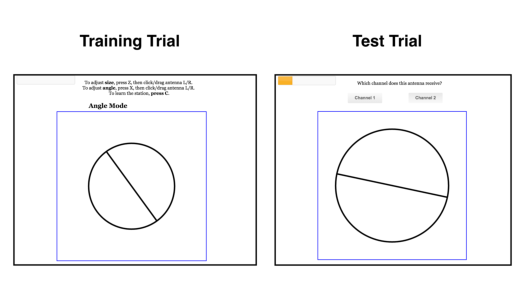
\includegraphics{figs/stimuli-1} 

}

\caption[The left panel shows a screenshot of the stimuli used in all experiments]{The left panel shows a screenshot of the stimuli used in all experiments. The right panel shows the true category distributions for the single dimension, Rule-Based category and the two dimensional, Information-Integration category.}\label{fig:stimuli}
\end{figure*}
\end{CodeChunk}

Figure 1 shows a screenshot of the stimuli used in all experiments.
Visual stimuli were black ``antennas'' on a white background. Each
antenna could vary along two continuous dimensions -- radius size or
central angle -- and was assigned a value between 1 and 600. These
values were converted to pixel values for display on a computer screen.
To ensure that participants could not complete a full rotation of the
antenna, the rotation of the central angle was limited to 150 degrees.
Finally, the minimum radius and angle values were randomized for each
participant, such that each participant was assigned a unique optimal
decision boundary.

Radius and angle values for the 96 passive training trials were
generated from two Gaussian distributions with identical mean and
covariance parameters as Markant \& Gureckis (2014) (see Figure 1). For
test trials, we created a uniform grid of 192 unique test items that
covered the entire feature space. We randomly sampled 8 items from each
quadrant to get 32 test trials for each block. We then randomized the
order of the training and test trials within each block for each
participant.

\subsubsection{Design and procedure}\label{design-and-procedure}

Participants saw a total of 288 trials (96 training trials and 192 test
trials) across 6 blocks. Each block consisted of 16 training trials and
32 test trials. Before starting the task, participants were told that
this was a game where they would see ``loop antennas'' for televisions
and each antenna received one of two channels (CH1 or CH2), and their
goal was to learn the difference between the two types of antennas. We
introduced some uncertainty by telling participants that the antennas
could pick up the wrong channel on occasion, and that they should learn
what channel is most often received by a particular type of antenna.

After the instructions, participants were randomly assigned to one the
two between-subjects conditions (Active vs.~Passive training). In the
Active training condition, participants were able to design their own
antennas to test. They modified the antenna by clicking and dragging the
mouse from left to right. To change the size of the antenna, they first
pressed the ``Z'' key. To change the angle, they first pressed the ``X''
key. When participants were finished with their design, they pressed the
spacebar to see which channel (Ch1 or Ch2) the antenna received. The
channel label appeared in a text box with a green border located above
the antenna.

In the Passive training condition, participants were shown antennas with
size and angles generated from the underlying category distributions.
After a two second delay they were told which channel the antenna
received. To ensure that participants saw the channel, they had to click
on the channel text in order to advance the experiment. When they
clicked the channel text, a green box appeared around the text to
indicate that their response had been recorded.

After completing the training, participants in both conditions proceeded
to the test trials. On each test trial participants saw an antenna and
were asked, ``Which channel does this antenna receive?'' To indicate
their response participants selected one of two buttons located above
the antenna.

\subsection{Results and Discussion}\label{results-and-discussion}

\subsubsection{Overall classification
accuracy}\label{overall-classification-accuracy}

\begin{CodeChunk}
\captionsetup{width=0.8\textwidth}\begin{figure*}[h]

{\centering 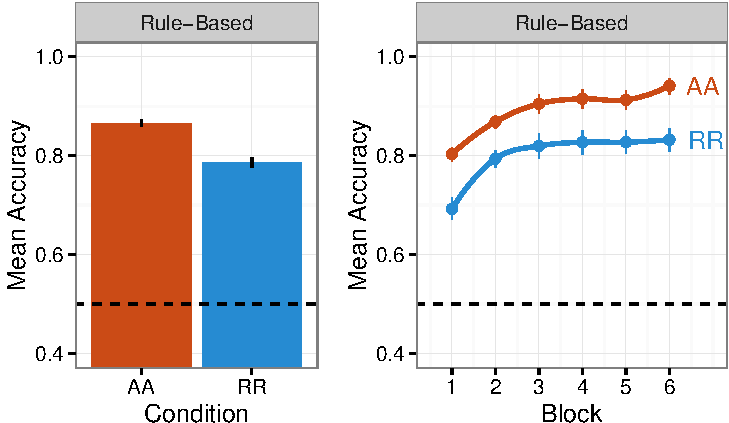
\includegraphics{figs/exp1a_acc-1} 

}

\caption[The left panel shows a screenshot of the stimuli used in all experiments]{The left panel shows a screenshot of the stimuli used in all experiments. The right panel shows the true category distributions for the single dimension, Rule-Based category and the two dimensional, Information-Integration category.}\label{fig:exp1a_acc}
\end{figure*}
\end{CodeChunk}

\subsubsection{Classification accuracy across
blocks}\label{classification-accuracy-across-blocks}

\subsubsection{Relationship between evidence selection and
learning}\label{relationship-between-evidence-selection-and-learning}

\section{Experiment 1b}\label{experiment-1b}

\subsection{Methods}\label{methods-1}

\subsubsection{Stimuli}\label{stimuli-1}

Stimuli were identical to Experiment 1a.

\subsubsection{Participants}\label{participants-1}

Participant recruitment and inclusionary/exclusionary criteria were
identical to those of Experiment 1 (excluded TODO HITs). TODO HITs were
posted for each condition (TODO) for total of TODO paid HITs.

\subsubsection{Design and procedure}\label{design-and-procedure-1}

\subsection{Results and Discussion}\label{results-and-discussion-1}

\section{Experiment 2}\label{experiment-2}

\subsection{Methods}\label{methods-2}

\subsubsection{Stimuli}\label{stimuli-2}

Stimuli were identical to Experiment 1.

\subsubsection{Participants}\label{participants-2}

Participant recruitment and inclusionary/exclusionary criteria were
identical to those of Experiment 1 (excluded TODO HITs). TODO HITs were
posted for each condition (TODO) for total of TODO paid HITs.

\subsubsection{Design and procedure}\label{design-and-procedure-2}

\subsection{Results and Discussion}\label{results-and-discussion-2}

\section{Experiment 3}\label{experiment-3}

\subsection{Methods}\label{methods-3}

\subsubsection{Stimuli}\label{stimuli-3}

Stimuli were identical to Experiments 1 and 2.

\subsubsection{Participants}\label{participants-3}

Participant recruitment, and inclusionary/exclusionary criteria were
identical to those of Experiment 1 and 2 (excluded TODO HITs). 40 HITs
were posted for each condition (TODO) for total of TODO paid HITs.

\subsubsection{Design and procedure}\label{design-and-procedure-3}

\subsection{Results and Discussion}\label{results-and-discussion-3}

\begin{table}[H]
\centering
\begin{tabular}{rrrrr}
  \hline
 & Estimate & Std. Error & t value & Pr($>$$|$t$|$) \\ 
  \hline
(Intercept) & 0.05 & 0.10 & 0.5 & 0.61 \\ 
  x & 2.10 & 0.11 & 18.5 & 0.00 \\ 
   \hline
\end{tabular}
\end{table}

\section{General Discussion}\label{general-discussion}

\begin{itemize}
\itemsep1pt\parskip0pt\parsep0pt
\item
  Recap findings

  \begin{itemize}
  \itemsep1pt\parskip0pt\parsep0pt
  \item
    Active learning advantage in a direct replication (yay science!)
  \item
    Passive-active better than Active-passive
  \item
    Conceptual replication
  \end{itemize}
\item
  Expand on why we see AR \textgreater{} RA

  \begin{itemize}
  \itemsep1pt\parskip0pt\parsep0pt
  \item
    Sequential hypothesis testing model
  \item
    Gain some understanding of task before exploring
  \item
    RA is bad because you can't refine your current hypothesis. Can only
    use the data you are given to confirm/reject current hypothesis
  \end{itemize}
\item
  Limitations

  \begin{itemize}
  \itemsep1pt\parskip0pt\parsep0pt
  \item
    AA was always best
  \item
    task analysis
  \item
    complexity of real world learning
  \end{itemize}
\item
  Takeaway point:
\end{itemize}

\section{Acknowledgements}\label{acknowledgements}

We are grateful to Doug Markant and Todd Gureckis for sharing the
details and code from the original experiment. We thank the members of
the Language and Cognition Lab for their helpful feedback on this
project. This work was supported by a National Science Foundation
Graduate Research Fellowship to KM.

\section{References}\label{references}

\setlength{\parindent}{-0.1in} \setlength{\leftskip}{0.125in} \noindent

Markant, D. B., \& Gureckis, T. M. (2014). Is it better to select or to
receive? Learning via active and passive hypothesis testing.
\emph{Journal of Experimental Psychology: General}, \emph{143}(1), 94.

\end{document}
